\documentclass[10pt,english]{article}
\usepackage[T1]{fontenc}
\usepackage[utf8]{inputenc}
\usepackage{lmodern,amsmath,amssymb,booktabs}
\usepackage{graphicx}
\usepackage[main=english]{babel}
\usepackage[letterpaper,margin=0.72in]{geometry}
\usepackage{xcolor,titlesec,microtype,xurl,hyperref,needspace}
\usepackage[skins,breakable]{tcolorbox}
\hypersetup{pdftitle={Why Subset-Sum Runtimes Form Several Bands},hidelinks}
\definecolor{paperink}{HTML}{26231F}
\definecolor{paperaccent}{HTML}{6E5943}
\definecolor{paperline}{HTML}{C8BCAD}
\definecolor{paperboxbg}{HTML}{F7F3EC}
\color{paperink}
\titleformat{\section}{\normalfont\sffamily\large\bfseries}{}{0pt}{\color{paperaccent}\rule{2pt}{1.05em}\hspace{7pt}}
\titlespacing*{\section}{0pt}{9pt}{4pt}
\tcbset{accentbox/.style={enhanced,breakable,colback=paperboxbg,colframe=paperline,boxrule=.45pt,arc=2mm,left=8pt,right=8pt,top=6pt,bottom=6pt}}
\setlength{\parindent}{0pt}
\setlength{\parskip}{4pt plus 1pt minus 1pt}
\setlength{\emergencystretch}{3em}
\setlength{\abovedisplayskip}{6pt plus 1pt}
\setlength{\belowdisplayskip}{6pt plus 1pt}
\newcommand{\E}{\mathbb E}
\newcommand{\Var}{\operatorname{Var}}
\newcommand{\Cov}{\operatorname{Cov}}
\begin{document}
{\LARGE\sffamily\bfseries Why Subset-Sum Runtimes Form Several Bands}\par
\vspace{3pt}
{\large\sffamily A route mixture from structural costs}\par
\vspace{6pt}
{\small Research note for \emph{Certified Coverage of Exponential Search Spaces}\hfill October 30, 2026}\par

\begin{tcolorbox}[accentbox]
\textbf{Question.} For each list of numbers and target, the subset-sum solver asks whether some
numbers add to the target; across hundreds of inputs, its runtimes pile up in
distinct bands instead of one smooth mound.
Why are the runtime bands separated and strikingly jagged?
The solver schedule gives an exact mixture over exit routes; the repo's core
bounds and OpenAI's deficiency measure suggest their cost scales. A smooth
lognormal mixture is a useful sketch, but its local failures pose a further
question about discrete solver behavior and the sampled inputs.
\end{tcolorbox}

\section{The measured object and an exact mixture}
An input $x=(w,t)$ consists of a list $w=(w_1,\ldots,w_n)$ of positive integer
weights and a target $t$; $n$ counts the listed items. The
histogram uses 576 unscaled targets on 144 generated lists, with
$n\in\{24,32,38\}$. The exact reference reduces the target, then tries a
filtered check, bitset, superincreasing-core enumeration, bounded depth-first
search (DFS), and meet-in-the-middle (MITM). It divides an $8L$ allowance
among methods, with state and bitset caps; $L$ is encoded input length and its
work units are not uniform bit operations. The horizontal variable $Y$ is
elapsed milliseconds, including earlier attempts, but excluding extraction
of saved machine-learning features.

Fix the input generator and solver policy; $\Pr$ refers to a draw of an input
under that choice. Let $R$ be the first route returning an exact answer, or
$\bot$ if every route stops without one. Write $\mathcal R$ for these exit
labels and $r$ for one label. For any set $A$ of elapsed times, conditioning
on the disjoint events $\{R=r\}$ gives
\begin{equation}
 \boxed{\Pr(Y\in A)=\sum_{r\in\mathcal R}\pi_r\Pr(Y\in A\mid R=r),
 \qquad \pi_r=\Pr(R=r).} \label{eq:route}
\end{equation}
For a uniform draw from the saved corpus, $\pi_r=N_r/576$, where $N_r$ is the
number of inputs exiting at route $r$. The counts
below come directly from the saved run traces, without estimating a density:
\begin{center}\small
\begin{tabular}{lrr@{\qquad}lrr}
\toprule
Exit route & $N_r$ & Median ms & Exit route & $N_r$ & Median ms\\
\midrule
Exact reduction & 129 & 0.013 & DFS & 205 & 2.64\\
Bitset & 49 & 0.065 & MITM & 30 & 8.72\\
Core enumeration & 17 & 0.668 & Unresolved stop & 146 & 12.36\\
\bottomrule
\end{tabular}
\end{center}
The filtered check makes no first completions. Each route's time includes
earlier attempts. The 146 unresolved values are stopping times; eventual
completion times are unknown. These six exit routes are not the six components
of the unconstrained lognormal fit.

\begin{figure}[!t]
\centering
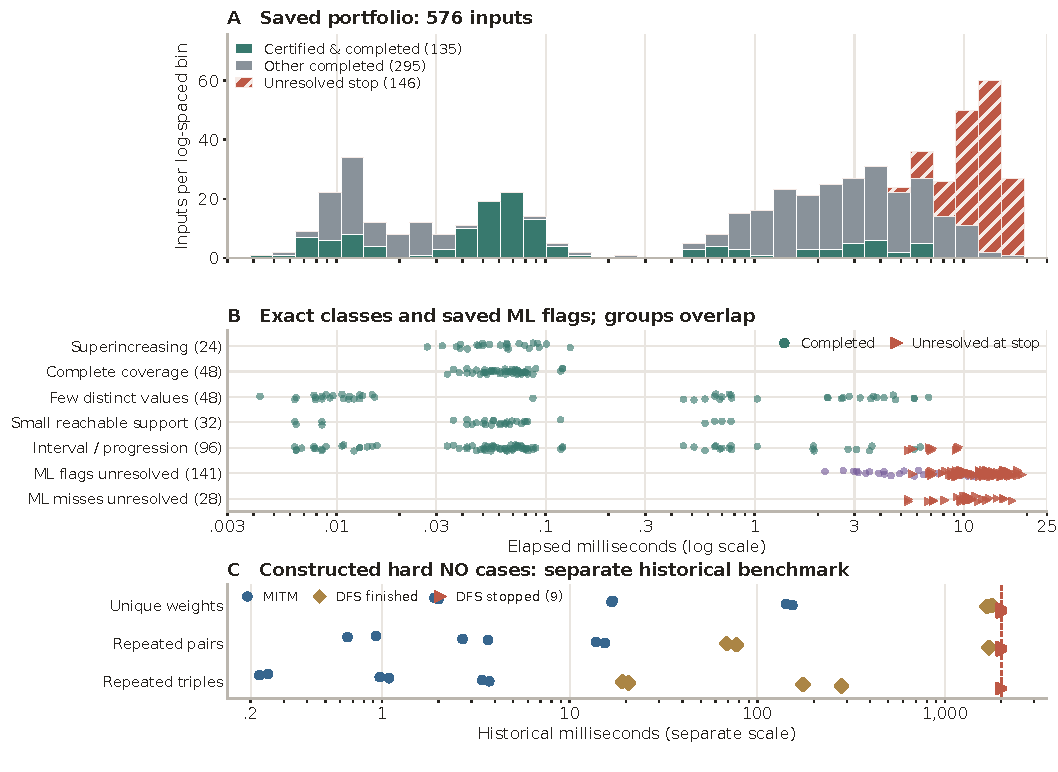
\includegraphics[width=\linewidth]{Runtime_Distribution_Histogram.pdf}
\caption{Saved elapsed times for the 576 unscaled inputs (A--B), with
log-spaced bins and exact-class or machine-learning (ML) markers. A circle
marks a completed input and a triangle an unresolved stop in B. The 18
constructed hard NO cases in C come from a separate historical benchmark
and use different solvers and a different horizontal scale.}
\label{fig:runtimes}
\end{figure}

Figure~\ref{fig:runtimes} shows why a single smooth law hides useful
structure. The fastest times cluster at exact reduction and bitset scales;
DFS, MITM and work-limited stops occupy later bands, though each time includes
earlier attempts. Exact class markers overlap because one input may satisfy
several certificates. Nine interval/progression inputs still stop unresolved
under this capped portfolio, so class membership alone does not guarantee
completion here. The ML flag is a saved prediction, not a certificate: it
flags 118 of the 146 unresolved inputs and also 23 completed ones. The
historical hard NO cases illustrate much longer DFS searches, but their
times cannot be pooled with the 576-input distribution.

\section{Completed times, rather than stopping times}
Let $D=\mathbf1\{R\ne\bot\}$ indicate an exact completion, where
$\mathbf1\{\cdot\}$ is one if its condition holds and zero otherwise; let
$T$ be $Y$ restricted to $D=1$. Conditioning~\eqref{eq:route} again gives, for any
time set $A$,
\begin{equation}
 \Pr(T\in A\mid D=1)=\sum_{r\ne\bot}q_r\Pr(Y\in A\mid R=r),
 \qquad q_r=\Pr(R=r\mid D=1)=N_r/430. \label{eq:completion}
\end{equation}
The top panel of Figure~\ref{fig:completion} isolates these 430 total completion times,
including earlier attempts. Its fast reduction/bitset cluster and later
DFS/MITM cluster are more distinct without the 146 stopping times. The
completed-input median is 1.00 ms; the unresolved runs cannot be assigned a
completion time. This is a conditional distribution for the capped solver,
not the eventual runtime law for all inputs.

\section{Coverage, exceptional sums and shared tables}
Note I accounts for $C(n)$ certified choices among the $2^n$ possible subsets
and $r_{\rm states}(n)=2^n-C(n)$ choices left for explicit search, paying
separately for representation and checking. Notes V--VI replace many
individual choices by one exact core query. Let $I$ be core indices and $E$
the disjoint exception indices, together covering all $n$ items. The decision
equivalence is
\begin{equation}
 t\in\mathcal A(I\cup E)
 \quad\Longleftrightarrow\quad
 \exists s\in\mathcal A(E):\ t-s\in\mathcal A(I),
 \qquad \mathcal A(V)=\Bigl\{\sum_{i\in S}w_i:S\subseteq V\Bigr\}. \label{eq:core}
\end{equation}
Here $\mathcal A(V)$ contains distinct sums from index set $V$, and $S$ is one
subset of it. Thus an exceptional sum leaves a target to query in the core.
If $e=|E|$, the implemented selection route may inspect up to $2^e$
exceptional assignments ($|E|$ counts indices), paying discovery cost $F$
and one core query each; a witness can stop it early. Note V's different exact
route merges equal exceptional sums, giving $K=|\mathcal A(E)|\le 2^e$
queries. OpenAI's deficiency is $d(E)=e-\log_2K$, where $\log_2$ is base two:
\begin{equation}
 K=2^{e-d(E)},\qquad
 T_{\rm V}=O\!\bigl(n\log(n+1)+(n+1)K\bigr)
 \quad\text{arithmetic operations}. \label{eq:deficiency}
\end{equation}
Here $T_{\rm V}$ is Note V's distinct-sum runtime; $O(\cdot)$ bounds growth up
to constant factors. Twelve equal exceptions give $K=13$, versus $2^{12}$
selections. OpenAI uses high deficiency for short sum lists and low deficiency
for many filterable representations. These are cost regimes, not input
probabilities.

\section{A shared table and a structural distribution}
Note VII adds a reusable geometric table with $H$ quotient rows and $W$
residual positions per row; $G$ bounds point tests per shifted target. If
$F$ pays preprocessing and discovery in bit operations, merging exceptional
sums gives
\begin{equation}
 T_{\rm combined}\le F+O^*\!\left(HW+2^{e-d(E)}(1+GW)\right).
 \label{eq:geom}
\end{equation}
Here $T_{\rm combined}$ is bit cost, and $O^*$ hides factors polynomial in
binary length $L$. The $HW$ term builds one table; $1+GW$ covers each
distinct sum's checks. The histogram's portfolio uses selection enumeration,
so these bounds do not equal its measured milliseconds.

The route identity~\eqref{eq:route} also applies to a hypothetical policy
using merged sums. On that route $r$, let discovery cost $a_r\ge0$ time units
and each query cost fixed $b_r>0$. Write
$p_{r,k}=\Pr(K=k\mid R=r)$ for the probability of $k$ distinct sums. The
proxy $Y_r=a_r+b_rK$ has conditional cumulative distribution
\begin{equation}
 \Pr(Y_r\le y\mid R=r)
 =\sum_{k\ge1}p_{r,k}\,\mathbf 1\{a_r+b_rk\le y\}.
 \label{eq:pushforward}
\end{equation}
Here $y$ is a time threshold and $\mathbf1\{\cdot\}$ is one when its condition
holds, zero otherwise. Combined with~\eqref{eq:route}, this is a discrete
mixture from structural support sizes. The implemented route instead depends
on selections visited; the geometric route also varies in $HW$ and point
tests. Equation~\eqref{eq:pushforward} describes its stated proxy, not the
saved clock readings.

\section{A smooth guess and the jagged remainder}
When query work dominates, model $T\simeq b_r2^{S_r}$, with $\simeq$ meaning
approximate cost. For merged sums $S_r=e-d(E)=\log_2K$; for full selection
enumeration $S_r=e$. Other routes need other drivers, such as bitset width,
DFS states or stored half sums. Allowing $b_r$ to vary across inputs, set
\begin{equation}
 Z_r:=\ln T\simeq\ln b_r+(\ln2)S_r \label{eq:logcost}
\end{equation}
where $\ln$ is the natural logarithm, $\exp$ its inverse, and logged times
are numeric values in milliseconds. If, as a separate
assumption, $Z_r\mid R=r$ is approximately normal with mean $\mu_r$ and
standard deviation $\sigma_r>0$, then $y=\exp(z)$, $dz=dy/y$, and
conditioning give the density
\begin{equation}
 f_{T\mid D=1}(y)\approx\sum_{r\ne\bot}q_r\frac{1}{y\sigma_r\sqrt{2\pi}}
 \exp\!\left[-\frac{(\ln y-\mu_r)^2}{2\sigma_r^2}\right],\qquad y>0.
 \label{eq:lognormal}
\end{equation}
For a histogram bin $(u,v]$, with $0<u<v$ in milliseconds, the expected
completed count is
\begin{equation}
 430\sum_{r\ne\bot}q_r\left[
 \Phi\!\left(\frac{\ln v-\mu_r}{\sigma_r}\right)-
 \Phi\!\left(\frac{\ln u-\mu_r}{\sigma_r}\right)\right],
 \label{eq:bins}
\end{equation}
where $\Phi$ is the standard normal cumulative distribution function. Equal
log-width bins therefore trace a mixture of normal curves on the $\ln y$
axis. The bottom panel of Figure~\ref{fig:completion} uses $q_r$ and route medians from the saved
runs, but chooses the five log-spreads by hand: it is a semi-empirical sketch,
not a parameter-free derivation or an optimized fit. In route order reduction,
bitset, core, DFS, MITM, its $\mu_r=\ln\tau_r$ uses median times
$\tau_r=(0.0132,0.0653,0.6676,2.6412,8.7183)$ ms and chosen
$\sigma_r=(0.45,0.60,0.75,0.70,0.50)$. The
query-dominated model gives
\[
 \mu_r=\E[\ln b_r\mid r]+(\ln2)\E[S_r\mid r],\quad
 \sigma_r^2=\Var(\ln b_r\mid r)+(\ln2)^2\Var(S_r\mid r)
       +2(\ln2)\Cov(\ln b_r,S_r\mid r).
\]
Here $\E$, $\Var$ and $\Cov$ mean conditional mean, variance and covariance;
``$\mid r$'' means given $R=r$. If acquisition $a_r$ matters, $T-a_r$ may be
lognormal instead. Discrete $K$, early witnesses, budget stops and sums of
paid stages can change the shape. Normality and the conversion from operation
counts to milliseconds require evidence. Separately, an earlier fit to all
576 observed elapsed times, including stops, compared 13 candidate families:
six lognormals scored best on held-out lists and four had the lowest Bayesian
information criterion (BIC), which penalizes parameter count. Those numbers
neither describe this completion-only sketch nor follow from~\eqref{eq:route}.

\begin{figure}[!t]
\centering
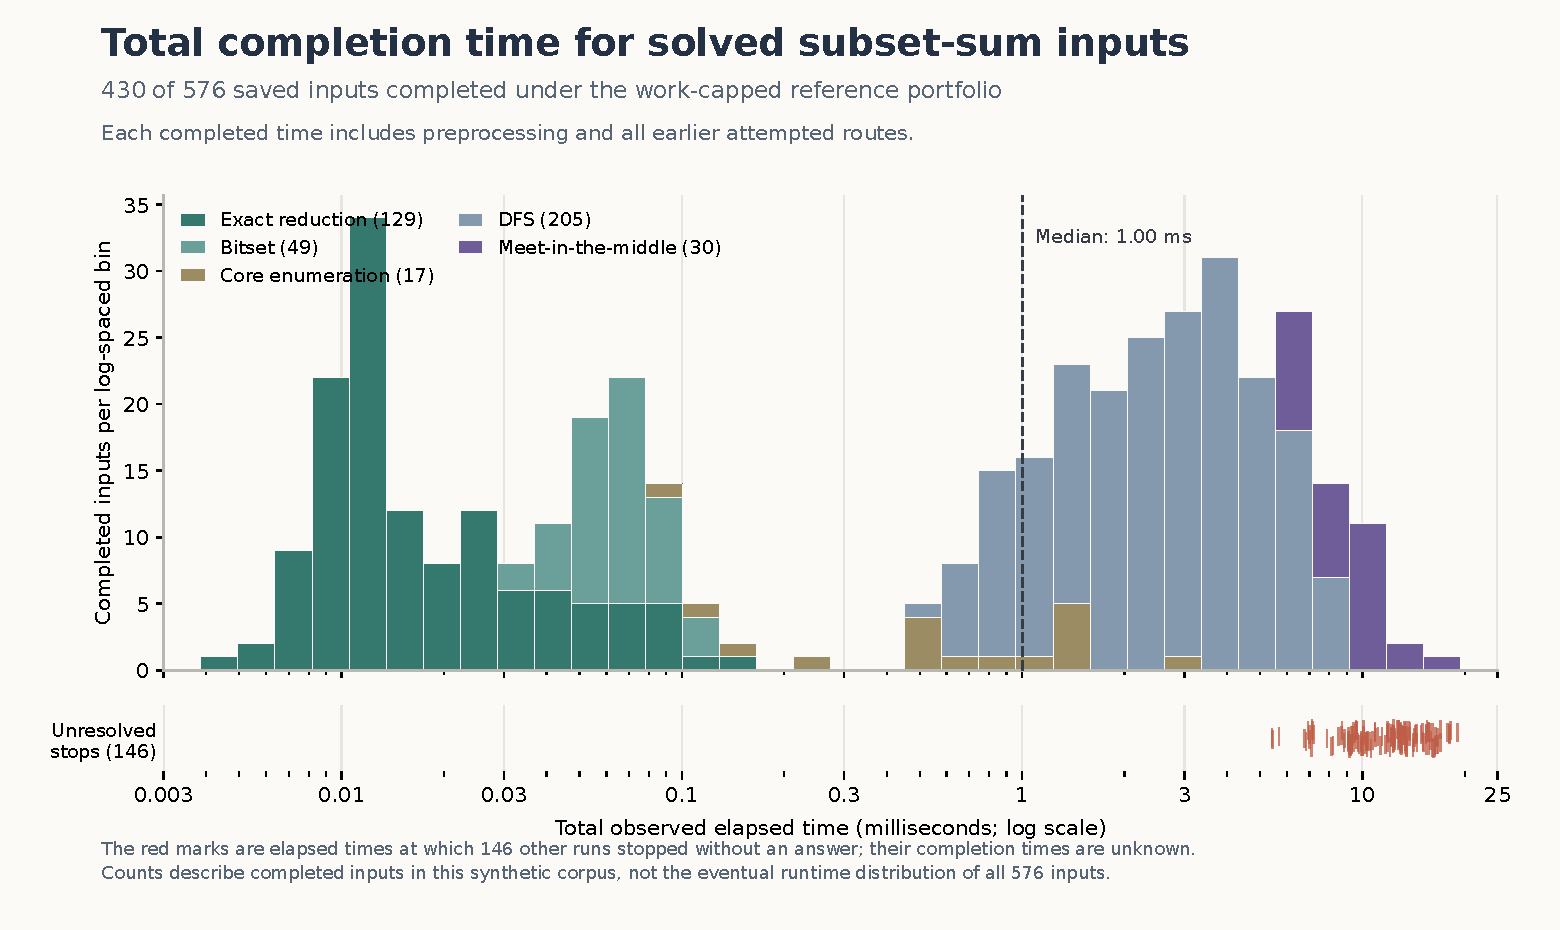
\includegraphics[width=\linewidth,trim={0 0.84in 0 1.12in},clip]{../Learned_Solvability_Subset_Sum/visualizations/runtime_histogram_20261030/subset_sum_completion_time_histogram.pdf}
\vspace{-4pt}
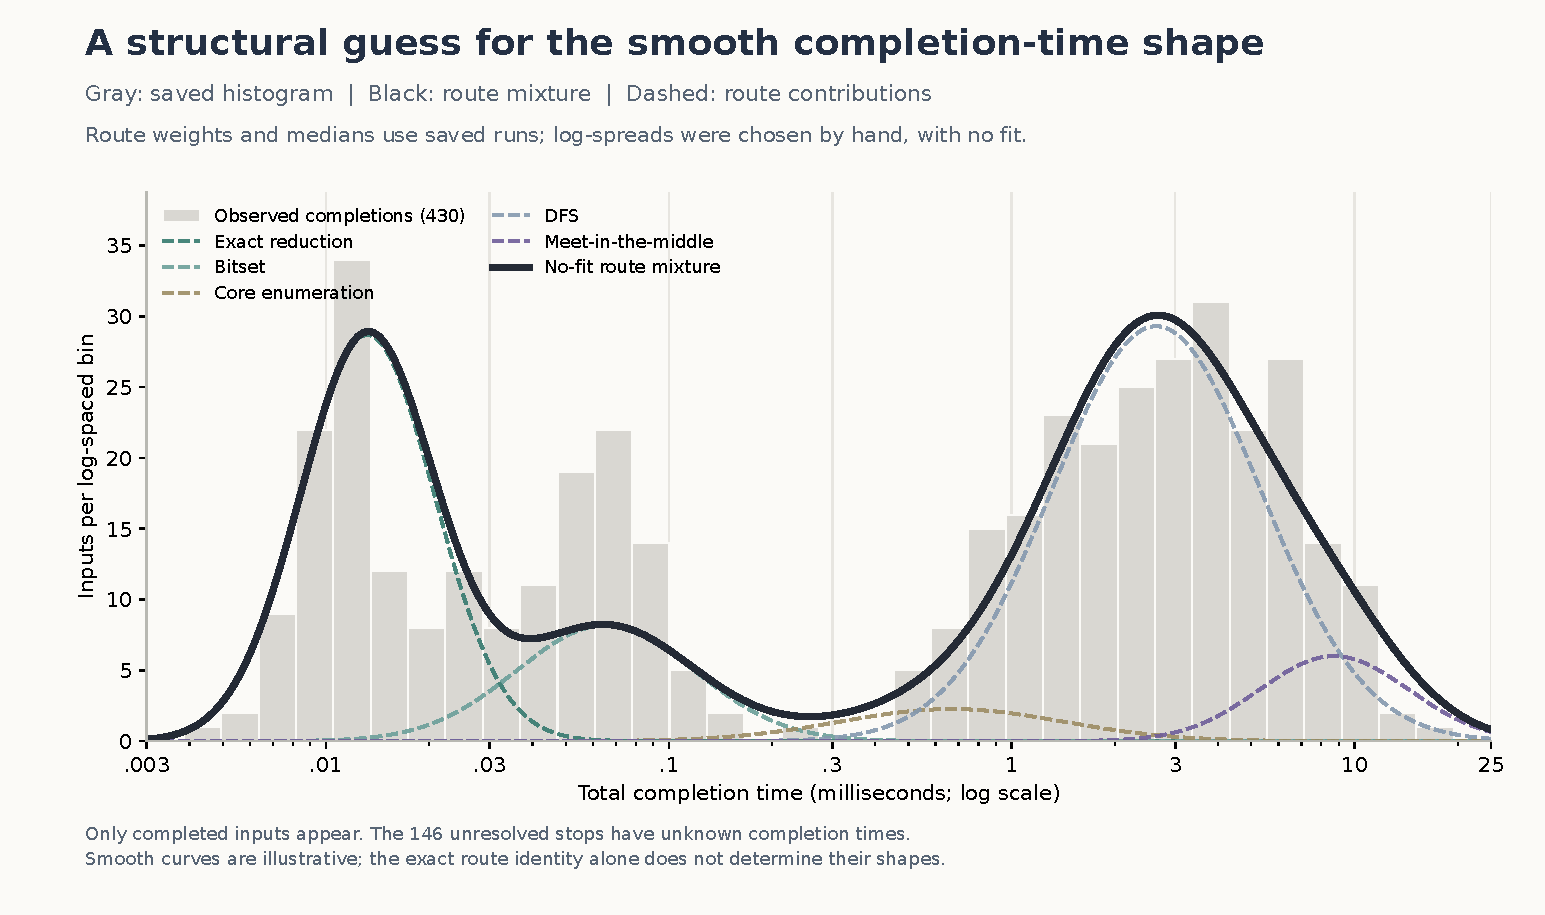
\includegraphics[width=\linewidth,trim={0 0.70in 0 1.12in},clip]{../Learned_Solvability_Subset_Sum/visualizations/runtime_histogram_20261030/subset_sum_analytical_completion_sketch.pdf}
\caption{Top: saved total times for the 430 completed inputs, colored by the
finishing route; red marks below are separate unresolved stopping times.
Bottom: the same observed counts in gray, with a hand-spread lognormal route
mixture in black and its components dashed. The curve captures broad bands,
but not every narrow spike or gap. Both panels use log-spaced bins.}
\label{fig:completion}
\end{figure}

\Needspace{9\baselineskip}
The puzzle is the jaggedness \emph{within} those broad bands. For bin $B_j$,
write $C_j=\sum_{i=1}^{430}\mathbf1\{T_i\in B_j\}$ for its observed count;
$i$ indexes completed inputs. If the inputs were independent with bin
probability $p_j$, its standard deviation would be
$\sqrt{430p_j(1-p_j)}$. Here targets sharing a weight list are dependent,
and discrete route switches, work caps and early witnesses may create real
thresholds. The smooth curve explains the envelope, but the visible spikes
and gaps could mix sampling variation with solver structure. Distinguishing
those explanations on fresh lists is an open empirical test, not a consequence
of the lognormal assumption.

OpenAI's October manuscript bounds every execution of a different randomized
solver by $O(2^{0.49n})$ word operations when input integer bit lengths are
polynomial in $n$. Its
small-support check, modular checksum and alias extraction are absent from
this portfolio. With no input distribution, that bound sets none of
$\pi_r,\mu_r,\sigma_r$. A no-fit test would derive route frequencies and
distributions of $e,K,HW$ and early stopping from the declared generator;
Equations~\eqref{eq:route} and~\eqref{eq:pushforward} would then predict an
operation-count histogram to check on new lists, including whether the
within-band irregularity persists.

{\footnotesize\textbf{Sources.} Repo:
\href{../Structural_Distance_Subset_Sum/THEORY.md}{Note V theory},
\href{../Learned_Solvability_Subset_Sum/docs/THEORY.md}{Note VI theory},
\href{../notes/07-geometric-cores/Runtime_of_Geometric_Core_Subset_Sum.pdf}{Note VII runtime companion},
\href{From_Choices_to_Sums.pdf}{From Choices to Sums},
\href{../Learned_Solvability_Subset_Sum/visualizations/runtime_histogram_20261030/README.md}{saved histogram}, and
\href{../Learned_Solvability_Subset_Sum/visualizations/runtime_histogram_20261030/distribution_fits/README.md}{fit analysis}.
OpenAI: \href{https://github.com/openai/math/blob/7ef5c0cc5ca4b0e072b7a050fca09ab24bc6fa3a/preprints/A-Low-Space-Algorithm-for-Worst-Case-Subset-Sum-September-26-2026/paper.pdf}{low-space manuscript}
and \href{https://github.com/openai/math/blob/7ef5c0cc5ca4b0e072b7a050fca09ab24bc6fa3a/preprints/Subset-Sum-in-Time-2-power-0-49n-October-4-2026/subset-sum.pdf}{$2^{0.49n}$ manuscript}, at the pinned revision.}
\end{document}
